\documentclass[]{article}
\usepackage[left=2cm,right=2cm,top=2cm,bottom=2cm]{geometry}
\usepackage[utf8]{inputenc}
\usepackage{amssymb}
\usepackage{amsmath}
\usepackage{graphicx}
\usepackage{hyperref}

\newcommand*{\poly}{\ensuremath{\mathbb{P}}}
\newcommand*{\real}{\ensuremath{\mathbb{R}}}
\newcommand*{\landau}{\ensuremath{\mathcal{O}}}

%opening
\title{Altklausuren: "Marketing Mix"}
\date{Sommersemester 2012 bis Sommersemester 2020}

\begin{document}
\maketitle

\begin{abstract}
Lösungen zu den Altklausuren der Vorlesung "Marketing Mix" am KIT. \\
\ \\
Viele ältere Klausuren haben noch andere Themen bzw. sind nicht als "Open-Book"-Klausur konzipiert. \\
Bei vielen Lösungen bin ich mir nicht sicher oder habe sie so beantowrtet wie ich die Frage verstanden habe, da gerne einen Pull Request stellen und diskutieren. \\
\end{abstract}

\begin{itemize}
    \item Markenkern: "Ein Gedanke der die Seele der Marke einfängt", kein einfacher Werbeslogan!
    \item Markennutzen: "Was bietet mir die Marke?", Aufteilung in symbolisch, funktionell und emotional
    \item Markenpersönlichkeit: Asssoziation der Marke mit menschlichen Attributen
    \item Markenpositionierung: 
        \begin{itemize}
            \item Relevanz: Nutzenmerkmale müssen sinnvoll sein
            \item Fit: Marke muss zur Zielgruppe passen
            \item Nachhaltigkeit: Position muss sich längerfristig halten können
            \item Differenzierung: Marke muss sich von anderen Marken abheben
            \item Prägnanz: Merkmale der Marke müssen prägnant sein
        \end{itemize}
    \item Familienmarken: Gruppierung mehrerer Produkte zu mehreren Marken
    \item Anpassung der Markenarchitektur
        \begin{itemize}
            \item Line Extension: Neue Produkte zusammen mit alten unter der selben Marke verkaufen
            \item Brand Extension: Marke auf andere Produktsparte transferieren
            \item Parallelmarken / Multibranding: Eine Partnerschaft mit einer anderen/neune Marke eingehen
            \item Neue Marke: Eine neue Marke für neue Produkte entwickeln
        \end{itemize}
    \item Brand Equity: Auf die Marke zurückzuführende, abweichende Kundenreaktion auf die Marketingaktivität
    \item Preissuche: Wie viel Zeit und Resourcen werden von Kunden aufgebracht um Preise zu vergleichen?
    \item Preisimage: Die individuelle Bewertung des Preisniveaus durch Kunden
    \item Preiswissen: Alle Informationen rund um den Preis
    \item Referenzpreis: Der Bezugspreis für andere Preise gleicher/ähnlicher Güter
    \item Preisschwelle: Preise ab denen die Preisbeurteilung sich sprunghaft ändert (zB 99€ auf 100€)
    \item Preisfairness: Beurteilung als legitimer Preis
    \item Dual-Entitlement-Prinzip: Kunden sowie Anbieter haben Ansprüche auf einen fairen Preis/fairen Gewinn, gerade wichtig bei Preiserhöhungen
    \item Mental Accounting: Jeder hat mehrere Unterkonten, auf die er Gewinne und Verluste verbucht.
    \item Kostenorientierte Preisbestimmung: Der Preis wird aus den Kosten heraus berechnet
    \item Kosten-Plus-Berechnung: Die gesamten Forschungs-, Produktions- und Marketingkosten werden mit dem erhofften Gewinn summiert und durch die erwartete Absatzmenge geteilt.
    \item Target Costing: Der Stückpreis und die Absatzmenge sind fest, die Produktionskosten werden so lange gesenkt bis Gewinn erwirtschaftet wird.
    \item Conjoint Analysis: Merkmale finden und ihre Ausprägungen feststellen, dann jedes Merkmal bewerten lassen um die wichtigen Merkmale zu finden
    \item Preisdifferenzierung: Gleiche oder sehr ähnliche Produkte werden verschiedenen Kunden zu verschiedenen Preisen angeboten
    \item Zahlungsbereitschaft: Den maximalen Preis den jemand bereit ist zu zahlen
    \item Personenbezogene Segmentierung: Segmentierung anhand von Personengruppen
    \item Mengenbezogene Segmentierung: Segmentierung über die Absatzmenge
    \item Räumliche Segmentierung: Lokal unterschiedliche Preise
    \item Zeitliche Segmentierung: Unterschiedliche Preise zu untersch. Zeiten/an untersch. Tagen
    \item Leistungsbezogene Segmentierung: Preispremium für besserer Leistungen
    \item Bundling: Verkauf von Produkten in einem Paket zu einem Vorteilspreis
    \item Preispromotionen: Zeitlich befristete Preisangebote
    \item Elaboration-Likelihood-Modell: Das Modell beschreibt die Auswirkungen von Werbung auf die Einstellung gegenüber dem Produkt
    \item Attitude towards the Ad: die (positive) kognitive und emotionale Einstellung zur Werbung
    \item Affect Infusion: Information, die den Entscheidungsprozess beeinflusst
    \item strategischer Bias: Die Vorstellungen und Überzeugungen des Unternehmens verfälschen den Befragungswert
    \item hypothetischer Bias: Dadaurch das bei einer befragung das Produkt nicht gekauft werden muss verfälscht sich das Befragungsergbnis
    \item Transaktionskostentheorie: Nutzung von Märkten verursacht Unkosten, aber diese können von Unternehmen reduziert werden (was selber wieder etwas kostet). Sind die Gesamtkosten niedriger als im Direktvertrieb, so bringt der Markt etwas.
    \item Breite des Vertriebs: (intensiv/selektiv/exklusiv) Die Anzahl an Vertriebspartnern für ein Produkt
\end{itemize}

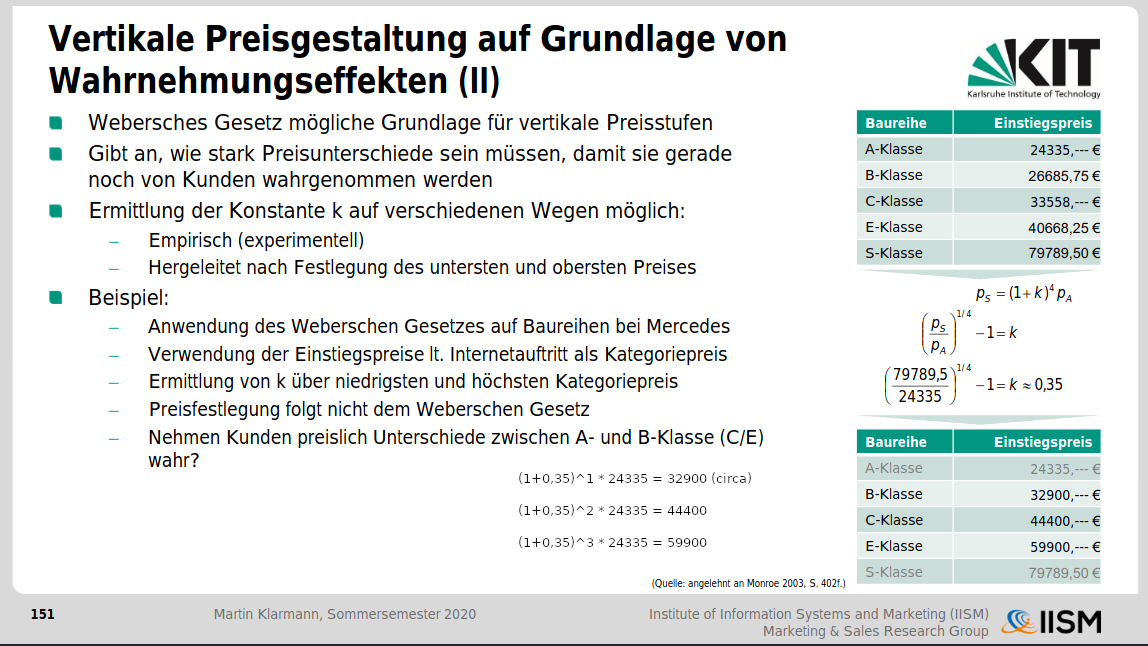
\includegraphics[width=\textwidth]{bilder/vertikale-preisgestaltung.png}

\newpage

\documentclass{article}
\usepackage[ngerman]{babel}
\usepackage[utf8]{inputenc}

\title{Sommersemester 2020 Hauptklausur}
\begin{document}
\maketitle


\section{Aufgabe 1}
\subsection{1.a}
Es handelt sich bei Dyson um Einzelmarkenstrategie. Dyson bietet einen Produkttyp (Staubsauger) an, ist aber einer der Marktführer in der eigenen Kategorie (Beutellose Staubsauger).


\subsection{1.b}
\subsubsection{segmentspezifische Ansprache}
Bezeichnet die Eigenschaft des Unternehmens, nur in einem bestimmten Segment an Waren, Vertreter zu sein. Bei Dyson könnte dieses Segment zB Haushaltsgeräte - Staubsauger sein. Für die Einzelmarkenstrategie von Dyson ist die segmentspezifische Ansprache sehr gut umsetzbar, da sie ja ausschließlich für das eine Segment produzieren.

\subsubsection{Ausstrahlungseffekte}
Sind zB Goodwill- und Treuetransfers, wie unter anderem das Payback Punkte-System. Die Nutzung solcher Effekte ist für die Markenstrategie von Dyson nicht von Vorteil, da ja nur innerhalb der eigenen Produktkategorie Treuetransfers stattfinden könnten, die wenigsten Kunden aber mehr als einen Staubsauger brauchen.


\subsection{1.c}
Bei der Einführung der Dyson-Leuchten hadelt es sich um eine Linienerweiterung. Da die Leuchten noch unter der Marke Dyson zu haben sind, jedoch nicht in der Produktkategorie wie Staubsauger zu finden wären, ist es eine neue Produktlinie in gleicher Marke.


\subsection{1.d}
Ein zentraler Erfolgsfaktor ist, eine Basismarke mit hoher Bekanntheit zu haben. Dies ist bei Dyson der Fall ist, da sie durch ihren langjährigen Vertrieb von Staubsaugern sehr bekannt sind. Da Leichten im weiteren Sinne wie Staubsauger auch Haushaltswaren sind, werden Kunden diese Marke beim Einkauf wiedererkennen.


\section{Aufgabe 2}
\subsection{2.a}
\subsubsection{Preissuche}
Bezeichnet die Bemühung eines Kunden, sich plattformunabhängig Preisinformationen über verschiedene Produkte zu suchen. Das Suchen online von Alternativen zu einem gewissen Produkt und Preisvergleiche zweier gleicher Produkte verschiedener Hersteller fallen unter anderem darunter.

\subsubsection{Preiswissen}
Umfasst sämtliche preisbezogene Infos, die im Langzeitgedächtnis eines Nachfragers gespeichert sind. Dies wird aufgeteilt in explizites Preiswissen, also die Preisinformation, an die sich der Nachfrager bewusst erinnert und in implizites Preiswissen, welches die unbewusste Anwendung gespeicherter Informationen zu einem Produkt bezeichnet.

\subsection{2.b}
Da die Kunden preissensibler agieren, suchen sie auch eher nach verschiedenen Preisen. Man kann also demnach einen generellen Anstieg bei potentiellen Kunden in der Preissuche voraussetzen und damit einhergehend auch, dass Nachfrager ein größeres Preiswissen haben, da sie sich vor dem Kauf/Nachfragen eingehend über das Produkt und Alternativen informiert haben.

\subsection{2.c}
Das Preisimage umfasst die käuferindividuelle Bewertung des Preisniveaus der Einkaufsstätte. Sekt Lidl die Preise schon vor der Mehrwertsteuersenkung, so kommt bei Kunden an, dass Lidl unabhängig von den staatlichen Beschlüssen, den Kunden Rabatte gönnen möchte. Somit steigt das Preisimage bei den Kunden, da Lidl als günstiger eingestuft wird, sich das Produktsortiment aber nicht verschlechtert hat.

\subsection{2.d}
Da Lidl zB ein großes Warensortiment hat, kann kein Kunde alle Preise kennen. Durch einzelne Eindrücke aus dem Sortiment bildet sich ein Kunde einen Eindruck vom Preisimage. Dabei spielen vor allem die Preisgünstigkeit und die Preiswürdigkeit eine große Rolle. Je größer das angebotene Sortiment ist, desto höher ist das Preisimage.
Lidl kann dies zB nutzen, indem sie häufig gekaufte Artikel reduzieren, sodass viele Kunden diese Rabattaktion mitbekommen. Somit stiege das Preisimage, da die ausgewählten und von vielen Kunden gekauften Artikel das Preisimage verändern.

\subsection{2.e}
Die Stategie "`Every-Day-Low-Price"', welche viele Discounter nutzen, baut darauf auf, alle normalen Preise des Warensortiments niedrig zu halten. Vor allem häufig Verkaufte Produkte werden standardmäßig zu "`Tiefpreisen"' (solchen, die unter den aktuellen Marktpreisen liegen) angeboten, sodass die Konkurrenz von Vollsortimentern durch das Preisangebot ausgeschlagen wird.
Preis-Promotions sind hingegen nur zeitlich begrenzte Angebote, zB Rabattaktionen auf einzelne Produkte, die den Absatz bei Händlern kurzfristig fördern. Diese können auch auf den Standardpreis von Discountwaren gezählt werden.

\subsection{2.f}
\subsubsection{Chance}
Eine Chance von Preis-Promotions ist die kurzfristige Erhöhung des Absatzes bei Edeka, da durch das Sonderangebot mehr Kunden einen Kaufzwang für das reduzierte Produkt empfinden und es auch kaufen, wenn sie es eigentlich nicht benötigen würden.

\subsubsection{Risiko}
Bei andauernden Preis-Promotions kann die Glaubwürdigkeit von Edeka sinken. Dann würden Kunden die Qualität der angebotenen Produkte infrage stellen, da diese ja die ganze Zeit zu "`Schleuderpreisen"' angeboten werden und lieber zur Konkurrenz gehen.

\section{Aufgabe 3}
\subsection{3.a} %LS: Hier bin ich mir nicht ganz sicher/ etwas halbherzige Begründung
eBays Suchmaschinenanzeigen greifen die Beobachter über die periphere Route an. Die Anzeigen motivieren browsende Personen, auf die Website zu gehen und bieten ihnen eine spontane Gelegenheit, sich abzulenken. Kunden nehmen die Information wahrscheinlich nur am Rande ihrer Aufmerksamkeit wahr, da sie damit beschäftigt sind, die Informationen der Suchmaschine zu verarbeiten. 

\subsection{3.b}
Da eBay ein Online Anbieter ist, sollte eBay Online-Werbung nutzen, um Neuerungen zu kommunizieren. Dadurch bietet sich auch der Vorteil, dass audiovisuell sehr präzise und zügig erklärt werden kann, was sich ändert. Außerdem können sowohl auf der eigenen Plattform, als auch auf hausfremden Websites Werbung geschaltet werden.

\subsection{3.c}
Die bezahlten und die regulären Klicks gehen im Zeitraum Anfang Juli 2012 bis Anfang August 2012 auseinander. Die blauen Werbeklicks liegen also nicht nur generell deutlich unter den Regulären, sondern verlieren temporär auch an Bedeutung.
Oder: Es sieht aus wie ein Tal vs. es sieht aus wie ein Berg???

\subsection{3.d}
Grundlegend geht es bei der "`Last Click"'-Heuristik darum, dass nur der letzte Klick auf die Werbung eines Werbenden in einer Suchanfragenkette eines Suchenden dem Werbenden auch monetär gutgeschrieben wird.
Hier würden die Suchwortanzeigen überschätzt werden, da diese offensichtlich nicht so ausschlaggebend für den Aufruf von eBay sind, wie die unbezahlten Verlinkungen.

\subsection{3.e}
Wenn die Google-Suchwortanzeigen komplett rausgenommen werden würden, würde sich das Muster wahrscheinlich nicht viel ändern. Da die unbezahlten Verlinkungen zu eBay ohnehin Überwiegen, würde die Plattform auch ohne bezahlte Suchwortanzeigen noch viele Klicks einfangen.

\subsection{3.f}
Aufgrund der eben genannten Faktoren, ist es für eBay nicht nötig, Suchwortanzeigen zu schalten. Das Unternehmen bekommt durch die unbezahlten Verlinkungen sogar mehr Klicks und kann sich durch das Auslassen von Suchwortanzeigen Geld sparen.

\end{document} 



%opening
\title{Sommersemester 2019 Nachklausur}
\maketitle


\section{Aufgabe 1}
\subsection{1.a}
    Das Modell der VL bezieht sich auf die Veränderung in Preis und Absatz wenn eine Marke dazu kommt. \\
    Dabei wird der Preis eines Produktes mit/ohne Marke verglichen und der Absatz eines Produktzes mit/ohne Marke verglichen. \\
    Aus der Differenz setzt sich der Markenwert zusammen.

\subsection{1.b}
    Die Marke "Amazon" hat einen höheren Markenwert als die Umsätze es suggerieren, da der Anteil der Marke zwar nicht viel am Umsatz geändert hat, aber die Kundenwahrnehmung der Marke stark gestiegen ist. \\
    Amazon erreicht dies durch stärkere Nutzung von Eigenmarken und dem Ausbau der Marke (Line extension).

\subsection{1.c}
    Das Kudnenwissen muss gleichzeitig spezifisch abgefragt und holistisch ermittelt werden. \\
    Dabei ist auch das oft nur implizite Markenwissen eine Herausforderung.
    %TODO Lösung

\subsection{1.d}
    Markenidentität ist der Eindruck der Marke, festgelegt anhand von Attributen und dem Auftreten. \\
    Amazon sieht sich als freundliches Unternehmen, dewegen ist ein lächeln im Logo vertreten.\\
    \ \\
    Markenerlebnis ist das Ziel, über alle Touchpoint gleich auftritt, man die Marke also immer gleich "erlebt". \\
    Das wird erreicht durch einen konsistenten Marketing Mix, bei Amazon zum Beispiel durch Werbung oder die preisliche einsortierung. \\

\subsection{1.e}
    Ein Konsistenter Markenauftritt ist sehr wichtig, damit man als Kunde direkt die gemerkten guten Assoziationen auf andere Produkte des Unternhemens überträgt und direkt weiß von wem dieses Produkt statt und was man davon erwarten kann. \\
    Dabei werden aber auch Badwill-Transfers ermöglich, also die Transferierung von negativen Assoziationen auf andere Produkte.

\subsection{1.f}
    Bei der Line extension werden neue Produkte zusammen mit bisherigen Produkten unter der selben Marke angeboten. So ist Amazon Music nur ein neues Produkt der Marke "Amazon".\\
    Bei der Brand Extension wird die Marke um weitere ähnliche amrken erweitert, unter welcher dann die neuen Produkte nagenboten werden. So ist Prime Video eine Marke welche ähnlich der Stammmarke Amazon ist (Prime aus dem Versand, Lächeln im Logo).
    Die alten Produkte werden dann weiterhin unter der alten Marken angeboten.


\section{Aufgabe 2}
\subsection{2.a}
    Die Kosten-Plus-Preisbildung folgt dem Prinzip: Wie viel soll das Produkt kosten? Und rechnet den Stückpreis aus, indem die Herstellungs- und Marketingkosten mit dem geplanten Gewinn addiert werden. \\
    Beim Target Costing gibt es schon einen festen Maximalpreis. Die Herstellungs- und Marketingkosten werden so angepasst, das bei diesem Preis noch Gewinn erzielt wird. \\
    \ \\
    Beides ist sehr schwer, da eine App keine Produktionskosten pro Stück hat und der Absatz nicht vorher festgelegt werden kann. \\

\subsection{2.b}
    Die direkte Kudnebefragung ist für die Migräne App gut geeignet. Aufgabe 2.a hat gezeigt dass es sehr schwer ist einen Preis für die App zu ermitteln. Durch dir Kundenbefragung wird der Preis in den Vordergrund gerückt, also wird das Preisbeusstsein sehr hoch sein. \\
    Problem ist dabei, dass VAriable Menge-Fragen nicht genutzt werden können und die Kunden von ihrem angegebenen Verhalten abweichen werden.

\subsection{2.c}
    Es handelt sich um personenbasierte Segmentierung. Jedem Kunden wird ein individueller Preis für die selbe Leistung angeboten. \\
    Der Algorithmus ermittelt damit die Merkmale der Kunden.

\subsection{2.d}
    \begin{enumerate}
        \item Monopol: Gegeben, da die Konkurrenzprodukte sehr geringer Nutzerzahlen aufweisen
        \item Nichtübertragbarkeit: Gegeben, da die App durch die Daten personalisiert wird. Ausserdem können IAP nicht weiter gegeben werden.
        \item Fair: Ggf. gegeben, hängt von der Einstellung des Algorithmus under der Einstellung der kunden ab
        \item Segmentierungmöglichekti: Durch den Algorithmus gegeben
        \item Verhältnismäßigkeit: wahrscheinlich nicht gegeben, App-Preise sind sehr gering und einen Algorithmus zu entwickeln ist nicht günstig.
    \end{enumerate}

\subsection{2.e}
    Die Grundidee der nutzenorientierten Preisbestimmung ist es, die für Kunden relevantesten Merkmale rauszufinden und auf Basis dieser Merkmale und einem Vergleichsprodukt den Preis zu bestimmen. \\
    Zwei Voraussetzungen sind ein Vergleichsobjekt/eine Referenz, welche hier aufgrund mangelnder Konkurrenz nicht gegeben ist und die Möglichkeit, Merkmale festzusetzen und ihre Ausprägung festzustellen. Dies ist hier gut gegeben.


\section{Aufgabe 3}
\subsection{3.a}
    Das Ziel des ELM ist es, die Auswirkung von Werbung auf die Einstellung von Kunden in 4 Wege grundsätzlich auf Basis von Involvement einzuteilen: \\
    Die zentrale route für hohes Involvement und die periphäre route für niedriges Involvement. \\
    Dazu kommt noch die Einteilung in die Grundlage der Einstellung: Affekt oder Koginition. \\
    \ \\
    Die Doir-Werbung wirkt auf der peripheren Route und arbeitet auf Grundlage von Kognitionen: Durch den gezeigten Star und Glamour wird eine einfache Überzeugung, dass Dior hochweertig ist und einen schön macht, erzeugt. \\

\subsection{3.b}
    Sex ist sexyy -> gut für den verkauf
    %TODO keine ahnung... sex ist immer gut dachte ich

\subsection{3.c}
    \begin{itemize}
        \item Aufmerksamkeit ist durch Werbepausen eher gering. Viele Leute gehen auch gerade dann auf die Toilette oder gucken zeitversetzt fern.
        \item Sinne: Es werden die audiovisellen Sinne angesprochen
        \item Handlungsbezug: Man sitzt vor dem Fernseher. Ohne aufzustehen, rauszugehen und einzukaufen ist kein Handlunsgbezug gegeben.
    \end{itemize}

    Die Dior-Werbung ist nicht besonders gut geeignet. Durch die MAsse an Beauty-Werbung geht die Werbung unter und ohne Handkungsbezug wird das Produkt nicht lange in den Köpfen der menschen bleiben.

\subsection{3.d}
    Das Fit zwischen Testimonial und Zielgruppe ist wie sich die Zielgruppe mit dem Testimonial identifizieren kann. \\
    Bei Charlize Theron ist dieses durch das Alter gegeben. Allerdings wird sich nicht jeder mit ihr idetifizieren können oder wollen. \\
    Alles in allem denke ich aber passt sie als Testimonial für eine Beautymarke sehr gut.

\subsection{3.e}
    %TODO Keine Ahnung
    \begin{itemize}
        \item "Nennen sie den NAmen dieser Marke"
        \item "Nennen sie die sechs bekanntesten Beautymarken"
        \item "Wie heißt die Werbeperson von Dior"
    \end{itemize}

    Ein weitere Methode wäre die Auswertung von Social Media Indikatoren
\documentclass{article}
\usepackage[ngerman]{babel}
\usepackage[utf8]{inputenc}

\title{Sommersemester 2019 Nachklausur}
\begin{document}
\maketitle


\section{Aufgabe 1}
\subsection{1.a}
Der Markenwert setzt sich aus dem Preispremium im Vgl. zu identischen Nicht-Markenprodukten + der zusätzlich verkauften Menge im Vgl. zu identischen Nicht-Markenprodukten zusammen.  

\subsection{1.b}
Das BrandZ-Rating orientiert sich nicht ausschließlich an den Umsätzen des Unternehmens, sondern berechnet die Brand Contribution mit ein. Da die Konsumentenmeinung ggü. Amazon im Jahr 2019 offensichtlich gestiegen ist, ist auch das BrandZ-Rating deutlich mehr gestiegen, als nur um die Gewinne, die Amazon in diesem Jahr eingefahren hat.
Zwei konkrete Maßnahmen Amazons, die in die Steigerung der Konsumentenmeinung und somit eine bessere Brand Contribution mit einspielen sind Amazons als hervorragend bewerteter Kundenservice und das ständig wachsende Angebot an Produkten und Dienstleisungen.

\subsection{1.c} kundenseitiges Markenwissen ermitteln
\subsubsection{1. Herausforderung}
Bei den Kundenbefragungen zur Brand Contribution werden sehr spezifische Dinge abgefragt, zu denen Kunden absolut unterschiedliche Meinungen haben können. Vor allem, da "`Verlangen"' und "`Bequemlichkeit"' sehr subjektive Werte sind.
\subsubsection{2. Herausforderung}
Amazon-Kunden haben ggf. kein konkretes Wissen über die Marke Amazon, sondern fühlen sich nur aufgrund emotionaler Werte, welche durch gutes Marketing von Seiten Amazons hervorgerufen werden kann, zur Marke hingezogen. Dies ergibt keine wertvolle Einschätzung der Qualität der Marke gegenüber.

\subsection{1.d}
\subsubsection{Markenidentität}
Die Markenidentität sind zB das stets gleich aussehende "`amazon"'-Logo mit dem Smiley-Pfeil, welches in allen Diensten zu erkennen ist, sowie auch die Typographie in den ebenfalls überall vorhandenen Slogans. Die Konsistenz innerhalb dieser Designentscheidungen generiert ein eindrückliches Bild, das bei Betrachtern direkt eine Assoziation mit der Marke "`Amazon"' hervorruft.

\subsubsection{Markenerlebnis}
Das Markenerlebnis spiegelt sich darüber wieder, dass Amazon in allen Diensten nicht nur ein einheitliches Auftreten hat, sondern sich auch inhaltlich gleich präsentiert. zB hat der "`Haupt-Dienst"' Amazon einen stärkeren Slogan als die anderen Serviced (video und music). Für die Streamingdienste ist allerdings auch inhaltliche Konsistenz vorhanden, da die Slogans, sowie auch die Logos, sich sehr ähneln. Somit wird den Kunden über alle Berührungspunkte das Bild "`Amazon"' vermittelt.

\subsection{1.e}
Dadurch, dass die Amazon-Services einen so hohen Wiedererkennungswert haben, bleibt die Erinnerung an die Marke im Gedächtnis eines Konsumenten länger hängen. Dieser muss sich nämlich nicht unterschiedliche Logos oder Slogans merken, sondern kann sich anhand der eingängigen amazon-Typographie und des Logos einfach dieses als Anhaltspunkt merken und wird so jeden Amazon-Dienst wiedererkennen.

\subsection{1.f}
"`prime video"' und "`amazon music"' sind beides Line Extensions, da sie den Namen der Hauptmarke enthalten und auch deren Image mit übernehmen, jedoch in einen anderen Produkt-Sektor gehören. Würden sie als komplett neue Marke verkauft werden, wäre dies eine Brand Extension.


\section{Aufgabe 2}
\subsection{2.a}

\subsection{2.b}

\subsection{2.c}

\subsection{2.d}

\subsection{2.e}

\subsection{2.f}


\section{Aufgabe 3}
\subsection{3.a} 
\subsection{3.b}

\subsection{3.c}

\subsection{3.d}
\subsection{3.e}

\subsection{3.f}

\end{document}



%opening
\title{Sommersemester 2019 Nachklausur}
\maketitle



\section{Aufgabe 1}
\subsection{1.a}
    Herr Bender bezieht sich auf den emotionalen Nutzen der Marke. Er verbindet die Marke Lufthansa und ihr Logo bzw. ihre Farbwahl mit Attributen wie souverän und vertrauenswüridg.

\subsection{1.b}
    Das sensorische Gedächtnis ist für die die Aufzeichnung von Sinneseindrücken verantowrtlich (zB die Farbe gelb hinterlässt einen warmen, freundlichen eindruck und die Interkation mit dem Flugpersonal lässt die Mitarbeiter sehr meschlich und freundlich wirken). Durch einen Lernproizess werden diese Eindrücke ins Kurzzeitgedächtnis übertragen, wo sie geübt werden. \\
    Am Endse werden die Informationen kodiert und die Assoziation (Lufthansa <-> freundlich) wird ins Langzeitgedächtnis übertragen.

\subsection{1.c}
    Die Markenidentität ist die Assoziation von menschlkichen Merkmalen mit einer MArke. Für Lufthansa ist die Identität wichtig, da sie als hochpreisige Airline unbedingt ein bestimmtes Image verkaufen muss, um sich von der Konkurrenz abzusetzen.

\subsection{1.d}
    Die DAchmarkenstrategie ist die Nutzung einer Marke für alle Produkte. \\
    Für ihre Tochtergesellschaften verwendet Lufthansa eigene Logos, da diese meist in einem anderen Preissegement liegen und durch Einzelmarken die Ansprache verscheiender Segemnte erleichtert wird. \\
    Gleichzeitig gibt es bei einer DAchmarke einen starken Goodwill-/Badwill-Transfer auf andere Produkten. Bei Einzelmarken ist dies sehr schwer. Für die Lufthansa beduetet dies dass das Image der Tochtergesellschaft nicht vom Image der Lufthansa abhängt. \\

\subsection{1.e}
    Es wurde der Wiedererkennungswert des Logos abgefragt.

\subsection{1.f}
    Da viele Leute das alte Logo kennen und sich die Form und Inhalt nicht geändert haben, werden auch viele das neue Logo erkennen. \\
    Allerdings kann es vorkommen, dass jemand sich am ehesten noch an die Farbe der LH errinnern kann. So jemand würde dann nach etwas gelben ausschau halten und würde damit das neue Logo nicht erkennen. \\
    So konnte man zum Beiospiel an einem überfüllten Flughafen noch irgendwo etwas gelbes sehen und sich daran orinitieren. Das geht jetzt nicht mehr. 



\section{Aufgabe 2}
\subsection{2.a}
    Es handelt sich um gemischstes Bundling. Beim Bundling werden mehrere Produkte zusammen verkauft (in einem sog. "Bundle"), bei der Spzialform des gemischten Bundles können diese Produkte auch einzeln erworben werden. \\

\subsection{2.b}
    Adobe will durch das Bundle erreichen, das man ggf. Software dazukauft, die man vorher nicht brauchte, wollte oder gar kannte. \\
    Die Adobe CC erreicht diese Ziel dadurch, dass es extreme Preisvorteile gibt, wenn man die Produkte im Bundle kauft und schon ab wenigen benötigten Produkten es Sinn macht, ein Abo über alle Apps abzuschließen.
    
\subsection{2.c}
    Sie würde nur InDesign kaufen. (gute wahl illustrator suckt nämlich HART im verlgiehc zu inkscape) \\
    Da ihre Zahlungsbereitschaft für Illustrator geringer ist als der Produktpreis, wird sie es nicht kaufen.

\subsection{2.d}
    %TODO

\subsection{2.e}
    Da die Preise bei einer direkten Kundenbefragung sehr in den Vordergrund rücken und damit verzerrt werden. \\

\subsection{2.f}
    \begin{itemize}
        \item Größe des Bundles: Ausprägung ist die Anzahl Produkte im Bundle
        \item Anzahl der Installationen: Auf wie vielen PCs dürfen die Produkte installiert werden? (1, 2 oder 3)
        \item Preis: Ausprägung sind verschiedene Preisschwellen (49€, 99€, 129€ bspw.)
    \end{itemize}



\section{Aufgabe 3}
\subsection{3.a}
    TV-Werbung erreicht generell sehr viele Leute, gerade bei Sportevents, welche nur im TV übertragen werden. Die Anzahl der erreichten Kontakte durhc Onlinewerbung hängt davon ab, wie oft die Werbung gezeigt wird. \\
    Die Präzision ist bei Onlinewerbung höher als bei TV-Werbung, da durch Nutzerprofile die Kontakte einzeln ausgewählt werden können.

\subsection{3.b}
    \begin{itemize}
        \item Werbebanner: Kleine Banner auf Webseiten mit statischem Inhalt, könnten zB Abbildungen neuer Schuhe zeigen.
        \item Werbevideos: Vor Online-Clips gezeigte kurze Werbevideos könnten kurze Spots von Läufern oder Fussballern zeigen
        \item Werbung bei Suchmaschinen: In den Ergbnissen von Suchmaschinen könnten bei der Suche nach "Sneaker" die Modelle von Adidas ganz oben stehen. 
    \end{itemize}

\subsection{3.c}
    A nutzt die zentrale Route, da nur interessierte Kunden sich den ganzen Text durchlesen werden. Durch gute Argumente wird der Kunde von der Werbung überzeugt. \\
    B nutzt die periphjere Route, da der Kunde nur kurz in den Kontakt mit dem Schuh kommt und nicht viele Informationen gezeigt werden. \\
    \ \\
    Die Printwerbung ist für die zentrale Route besser geeignet, da sie größer gedruckt werden kann. \\
    Bei Onlinewerbung ist meist nur ein kleiner Teil für die Werbung reserviert, das Involvement ist auch sehr viel geringer, da Onlinewerbung als besonders störend empfunden wird.

\subsection{3.d}
    Nein, da wie bereits gesagt Printwerbung nicht für die kleine Fläche geeignet ist. Das Involvement ist zu gering und der Text zu klein. 

\subsection{3.e}
    Durch die Messung von Clicks auf die Werbung kann sehr gut gemessen werden, wie gut die Werbung funktioniert. \\
    Bei der Werbung B könnte beim Click auf "Shop Boost" ein Cookie gesetzt werden, welcher dem Shop verrät wie man auf die Siete gekommen ist.



%opening
\title{Sommersemester 2019 Nachklausur}
\maketitle



\section{Aufgabe 1}
\subsection{1.a}
    Airbnb ist allgemein im Niedrigpreissektor anzutreffe. Man kriegt fast keinen Service, dafür sind die Preise pro Übernachtung sehr günstig. \\
    Airbnb Plus würde ich im mittleren Preissegment sehen. Man kriegt mehr Leistung und Sicherheit als bei den niedrigen Preisen des "allgemeinen" Airbnb, es ist aber noch keine Luxus-Unterkunft. \\
    \ \\
    Ich denke die Position wird sich nicht halten lassen, da die Hotelbranche zu ähnlichen Preisen einen besseren und persönlicheren Service bietet als Airbnb Plus. \\

\subsection{1.b}
    Ein konsistenter Markenauftritt ist wichtig, da nur durch Übung, Erinnerung und Assoziation eine Information im Langzeitgedächtnis bleibt. \\
    Es muss also immer wieder durch einen konsistenten Auftritt eine Kodierung der Information im Hirn erreicht werden.

\subsection{1.c}
    Airbnb Plus soll ein anderes Segment an Kunden bedienen als Airbnb. Dazu wird die Preisdifferenzieung auf Basis der Leistung angewandt. Mit Airbnb Plus erhält man besseren Service als bei Airbnb normal. \\
    Ausserdem kann räumlich Differenziert werden: Wenn die besten Wohnung im Stadtzentzum alle mit Airbnb Plus angeboten werden, ist man dazu geneigt den Service zu nutzen um so eine Wohnung zu bekommen.
    %TODO stimmt das so?

\subsection{1.d}
    Die MArkenidentität ist die Assoziation der Marke mit menschlichen attributen (freundlich, nett, sportlich, etc.) \\
    \ \\
    Das Markenerlebnis ist der Auftritt der Marke nach Außen, zB durch Verpackung, angebotene Leistung, Farben, Logo. \\
    \ \\
    Die Identität von Airbnb ist nicht besonders zuverlässig. "billig" und "unsicher" sind in meinen Augen Hauptattribute der Marke Airbnb. \\
    Das passt nicht zum geplanten Erlebnis, bei dem man durch komptente Mitarbeiter betreut werden soll und vorher durchgecheckte Wohnung angeboten bekommt.

\subsection{1.e}
    Airbnb Plus zielt hauptsächlich auf die Risikoreduktion ab. Wie in Aufgabe 1.d) erläutert wird das Angebot von Airbnb als nicht besonders sicher oder zuverlässig angesehen. \\
    Durch die Betreuung durch Mitarbeiter und der vorherige Check-Up der Wohnung wird das risiko, ein schlechtes Produkt zu erhalten, reduziert.



\section{Aufgabe 2}
\subsection{2.a}
    Die Kosten-Plus-Preisbildung nimmt alle Kosten (Produktion, Rohstoffe, Transport, Werbung) und den geplanten Gewinn, addiert diese auf und teilt sie durch die erwartete Absatzmenge. \\
    So wird der Preis pro Einheit errechnet. \\
    Ein Vorteil ist die sehr Transparente Preiserstellung, der Preis wird also sehr fair angesehen. Auf der anderen Seite wird so das "over-engineering" nicht berücksichtigt, welches sich negativ auf den Preis auswirken kann.

\subsection{2.b}
    Durch eine direkte Kundenbefragung mit offenen und geschlossenen Frageformen kann die Zahlungsbereitschaft abgefragt werden. Dabei werden den Kunden Fragen zum Produkt und zum Preis gestellt,
    bspw. "Würden sie das Produkt zu einem Preis von xx€ kaufen?" (geschl.) oder "Was ist der maximale Preis in € bei dem sie das Produkt noch kaufen würden?" (offen)

\subsection{2.c}
    Referenzpreise sind die Preise vergleichbarer Konkurrenzprodukte, an denen man das Preisniveau ablesen kann. \\
    Als Referenzpreis kann das Trikot eines anderen Fussballvereins gesehen werden. Problem bei Referenzen von Triokots sind, dass die jeweiligen Trikots hauptsächlich in einem Land verkauft werden
    (zB brasilianische Triokots in Brasilien) und sich die ZBs der einzlnen Länder stark unterscheiden.

\subsection{2.d}
    Ja, da das Trikot sich nächstes Jahr wieder ändern wird kann der zentrale Vorteil von Preispromos genutzt werden, nämlich der erhöhte Absatz der trikots zu günstigen Preisen. \\
    Der Nachteil, dass das Preisniveau sinken wird und Kunden die Waren nur im Angebot kaufen besteht eher nicht, da nächste WM jeder wieder ein Trikot zu Beginn des Cups braucht.

\subsection{2.e}
    Die Preisfairness ist die Einschätzung des Preises durch den Kunden. \\
    Der Kunde erẃartet dass der Anbieter ihm ein gutes Angebotr macht, gesteht dem Anbieter aber auch die Absicht ein, 
    Gewinn zu machen. So muss ein Preis gefunden werden, welcher für beide Seiten nachvollziehbar ist.

\subsection{2.f}
    Wie in der e) bereits genannt, sieht jede Seite es als ihr Recht an, einen guten Deal zu finden. \\
    Preiserhöhungen ohne erhöhte Unkosten durch den Anbieter werden allgemein als unfair angesehen. 
    Da Adidas aber betont, die Kosten der Produktiuon eines Trikots haben sich erhöht, 
    kann der Preis gerechtfertigt werden und wird damit wieder als fair angesehen.



\section{Aufgabe 3}
\subsection{3.a}
    Influencer-Marketing nutzt sog. Influencer, Social Media Nutzer mit großem Impact, um die Kaufentscheidungen von Kunde zu steuern. \\
    Dabei ist der Vorteil, dass die Influencer aus Kundensicht als Person aus "unserer Mitte" gesehn werden. Dadurch steigt ihre Glaubwüridgkeit.
    So ist das auch bei Bibi und MK.

\subsection{3.b}
    Durch den Klick auf einen Affiliatelink kann sehr gut gemessen werden, woher die Kunden kommen. \\
    Es ist in etwa so wie ein Aktionscode, nur hat der Kunde nichts davon.

\subsection{3.c}
    TV-Werbung, denn durch die Nutzung eines guten TV-Spots kann auch eine emotionbale Assoziation erreicht werden. \\
    Aussenwerbung, denn auch diese setzt auf die periphere Route durch bloßen Kontakt mit der Marke. \\
    
\subsection{3.d}
    Nein, da Bibi nicht gut zur hochpreisigen Marke MK passt. Bibi passt gut zu ihrer Zielgruppe, da dies aber meiste Kinde rund Jegendliche ohne Geld sind passen diese nicht zu MK. \\
    Die Zielgruppe von MK sind junge Erwachsene mit zu viel Geld, diese werden aber nicht die Videos von Bibi angucken.

\subsection{3.e}
    Der Trouble-Faktor ist das risiko bei der Nutzung eines Testimonials. 
    Es beschreibt die Möglichkeit dass das Tesitmonial etwas macht, was die öffentliche Meinung von ihm verschlechtert.
    Ein Beispiel anhand von Bibi wäre zum Beispiel wenn sie ihren Partner betrügt und das öffentlich wird. Das Image von Bibi nimmt Schaden und damit auch das Image von MK.

\subsection{3.f}
    Die Chance der Wiedererkennung der Marke steigt, wenn die Marke eine starke Präsenz hat. Bei einer Marke, welche Lifestyleprodukte anbietet, ist dies sehr wichtig. Product Placement ist dabei eine sehr kostengünstige Methode, eine hohe Bekanntheit der Marke zu erreichen.\\
    Gleichzeitig passt das Product Placement nicht unbedigt zum Image der Exklusivität der Luxusmarke MK. Wenn jeder mit den Produkten rumrennt spricht das nicht für eine besondere Exklusivität. \\
    \ \\
    Wenn das Placement gut geregelt ist und nicht zu aufdringlich kann es gemacht werden. Das Risiko des Verluistes der Exklusivität überwiegt in meinen Augen allerdings den Vorteil günstiger Werbung durch PP.



%opening
\title{Sommersemester 2019 Nachklausur}
\maketitle



\section{Aufgabe 1}
\subsection{1.abc}
    %THEMA LEbens zyklus

\subsection{1.d}
    Der Markenkern ist das zentrale Element der Marke, in etwa so wie das Motto, aber weniger auf einen slogan beschränkt sondern mehr als grundsatz der marke verstanden.

\subsection{1.e}
    Die Elektromobilitätsstrategie von BMW in Verbindung mit dem Markenkern sollte darauf abzielen zu zeigen, dass man auch fahrspaß mit Elektroautos haben kann.

\subsection{1.f}
    Die Markenarchitektur eines Unternehemens ist die Zurodnung von Produkten zu den Marken und die Beziehungen von den Marken unterinander (zB Tochtermarke)

\subsection{1.g}
    


%opening
\title{Sommersemester 2017 Hauptklausur}
\maketitle



\section{Aufgabe 1}
\subsection{1.abcdef}
    %THEMA Komplexitöätskosten, Opportunitätskosten, Verschiebung der Komplexität auf spätere Wertschöpfungsstufen



\section{Aufgabe 2}
\subsection{2.a}
    %TODO strategische bias hypothetischer bias
    Der strategische Bias ist die Überschätzung des Produktes und der damit verbundenen ZB. \\
    Der hypothetische Bias ist die Verzerrung der ZB durch die Befragten, da man in der Befragung das Produkt nicht wirklich kaufen muss.

\subsection{2.b}
    Der hypothetische Bias geht bei der Conjoint-Analyse herunter, da diese das Kaufverhalten durch die Merkmale und Ausprägungen besser darstellt. \\
    Ganz verschwinden tut er nicht, da auch hier wieder ein Unterschied zwischen wahren Kaufverhalten und angegebenem Kaufverhalten stattfindet.

\subsection{2.c}
    \begin{itemize}
        \item Sensorgröße: APSC oder 35er Vollformat
        \item Auflösung: 36MP, 20MP, 24MP
        \item AF-Pkte.: 51, 33, 45
        \item Bilder/sek.: 8, 4, 6
        \item Anbindung: Wifi, Wifi+BT, Wifi+BT+NFC
        \item Preis: 1000€/1500€/2000€, 2200€, 900€
    \end{itemize}

\subsection{2.d}
    Bei allen Merkmalen sind die Konkurrenzprodukte abbildbar.
    Jedoch hat ein Vollformatsensor standardmäßig eine höhere Auflösung als ein APSC, diese beiden Merkmale sind also gänzlich nicht unabhängig voneinander.

\subsection{2.e}
    %THEMA malen

\subsection{2.f}
    Gesamtnutzen Gewicht: 4,5
    %TODO

\subsection{2.g}
    %THEMA Luce Modell



\section{Aufgabe 3}
\subsection{3.a}
    Die Platzierung im Super Bowl-Finale ist für die Kontakte nicht zu übertreffen: Der Superbowl ist das größte Event im amerikanischen Fernsehjahr. \\
    GTleichzeitig sinkt dadurhc auch die Präzision: Sehr viele unterscheidliche Menschen gucken den Super Bowl, dadurch auch ein großer Teil der nicht Teil der Zielgruppe ist. \\
    Laut Text zielt die Werbung auf Frauen ab, der Streuverlust ist also auf den ersten Blick sehr hoch.
    Da der Super Bowl ein Sportevent ist, ist die erreicht Gruppe wahrscheinlich hauptsächlich männlich. \\
    \ \\
    Diese Streuverluste sind irrelevant, da für das Produkt Männer die Zielgruppe sind, auch wenn die Werbung anscheinend auf Frauen ausgelegt ist. \\

\subsection{3.b}
    Shampoo ist für mich auf jeden Fall ein low involvement Produkt. Die Nutzung von Huimor macht hier Sinn. \\
    Andererseits ist die Zielgruppe von Old Spice nicht auf junge Menschen ausgelegt, der Bildungsstand ist hierbei auch irrelevant. Der Humor passt nach diesem Merkmal also nicht so gut\\
    Humor passt auch zu den meisten Zielgruppen also wird es wohl auch auf die Kultur der Männer passen. (was ist das für eine frage bitte was ist die kultur deiner zielgruppe wenn deine zielgruppe FÜNFZIG PRIZENT ALLER LEBENDEN MENSCHEN IS ???)

\subsection{3.c}
    %THEMA Sex als Verkaufsargument

\subsection{3.d}
    Es wurde der Aided Recall abgefragt. \\
    Eine andere Methode ist die Abfrage der Dominanz, also ob die Marke die einzig bekannte Shampoo-Marke ist.

\subsection{3.e}
    %THEMA STAS Differenzial



\section{}



%opening
\title{Sommersemester 2014 Hauptklausur}
\maketitle


\section*{Aufgabe 1}
\subsection*{1.abcd}
    Nicht gefunden

\section*{Aufgabe 2}
\subsection*{2.a}
    Target Costing ist die Festlegung eines maximalen Verkaufspreises und die Anpassung der Produktions- und Marketingkosten an diesen Preis, sodass noch ein Gewinn erwirtschaftet wird. \\
    Auf der anderen Seite ist Kosten-Plus-Verfahren: Hierbei wird der Preis aus der Summe der Produktions- und Marketingkosten sowie dem Gewinn errechnet.

\subsection*{2.b}
    \begin{itemize}
        \item Billigprodukt: $5+3+0+0+0+22 = 30$
        \item A5000: $10+2+3+1+3 = 19$
        \item Luxusprodukt: $20+8+6+0+3+2 = 39$
    \end{itemize}

    Mit den Teilnutzenwerten 22 und 2 und den Preisen 200 und 600 würde ich einen Preis anstreben, der in der Mitte liegt: 12 Nutzenwertpkte. \\
    Das entspräche einem Preis von 400€.

\subsection*{2.c}
    Eine Conjoint Analysis als Preisgrundlage ist nicht sinnvoll. Bei der conjoint Analysis werden nur vordefinierte Merkmale betrachtet, ggf. sind das gar nicht die Merkmale die den Kunden wirklich wichtig sind. \\
    Ausserdem wird der Preis als Merkmal in den Hintergrund gerückt, was das Preisbewusstsein der Befragten schwächt.

\subsection*{2.d}
    Die direkte Kundenbefragung, dabei werden die Preise genau beachtet, was bei einem Haushalktsgerät wie einem Kühlschrank auch sehr typisch ist. \\
    Durch offene Frameformen kann ein guter Preis auch valide geschätzt werden. Das Problem des Variable Menge-Falls tritt bei Kühlschrankkäufen eigentlicha uch nicht ein.

\subsection*{2.e}
    Der durchweg höchste Teilnutzen ist der Inhalt (in L). bei 2 von 3 Produkten liegt der Wert für den Inhalt über allen anderen Werten

\subsection*{2.f}
    %THEMA habe ich nicht gefunden
    %Langfristig  möchte  die  Firma  Eiszeit  neue,  innovative  Produktideen  umsetzen,  um nicht  den  Anschluss  an  Konkurrenten  zu  verlieren. Welches  unternehmensexterne Verfahren  zur  Generierung  neuer  Produktideenist  hier  am  besten?Was  sind  jeweils zwei Vor-und Nachteile? (3 Punkte)


\section*{Aufgabe 3}
\subsection*{3.a}
    %TODO Skizze einfügen
    Das ELM hat 2 Wege, den primären und den periphären Weg: \\
    Welcher Weg genommen wird um die Einstellung von Kunden zu ändern hängt von der Motivation des Kudnen ab, sich mit dem Produkt zu beschäftigen. \\
    Bei high involvemtn wird der primäre weg genommen, bei low involvement der periphäre.

\subsection*{3.b}
    Motivation, Fähigkeit, Gelegenheit ... 
    \begin{itemize}
        \item mehr: zentrale Route
        \item weniger: Periphäre Route
    \end{itemize}

    Grundlage der Einstellung ... 
    \begin{itemize}
        \item Affekt
        \item Koginitonen
    \end{itemize}
    \ \\
    Die Nivea-Werbung ist eine positive Einstellung zur Kommunikationsmaßnahme, die Werbung soll emotional verarebitet werden. \\
    Die TecXL-Werbung arbeitet auf Grundlage von Kognitionen. Mit guten wertbasierten Argumenten, glaubhaft präsentiert.

\subsection*{3.c}
    Die Nivea-Werbung ja, die TecXL-Werbung ist zu klein geschrieben mit zu viel Informationen. Bei der Nivea-Werbung ist nur nicht ganz klar wofür geworben wird.


\section*{Aufgabe 4}
\subsection*{4.abc}
    %THEMA Informationsasymmetrie

\subsection*{4.de}
    %THEMA Mitarbeitermotivation




%opening
\title{Sommersemester 2013 Nachklausur}
\maketitle


\section*{Aufgabe 1}
\subsection*{1.abcd}
    Bassmodell kann nicht gefunden werden

\subsection*{1.e}
    \begin{itemize}
        \item Dachmarke
        \item Markenfamilie
        \item Einzelmarken
    \end{itemize}

    \begin{itemize}
        \item Positiv: Höhere Bekanntheit der Marke durch verstärktes Auftreten
        \item Positiv: Goodwill wirkt sich auf alle Produkte aus
        \item Positiv: Designs von Verpackungen können zT wiederverwendet werden (Resourcenschonend)
        \item Negativ: Badwill-Transfer
        \item Negativ: Produkte können nur eingeschränkt spezifisch profiliert werden
    \end{itemize}

\subsection*{1.f}
    Produktdiffusion??

\section*{Aufgabe 2}
\subsection*{2.a}
    SMART-Kriterien??

\subsection*{2.b}
    Ergebnisziele?? Verhaltensziele??


\section*{Aufgabe 3}
\subsection*{3.a}
    Kosten-Plus-Pricing startet mit den Herstellungskosten und addiert auf diese alle sonstigen entstandenen Kosten und den geplanten Gewinn obendrauf. \\
    Mit der geplanten Absatzmenge wird damit der Preis pro Einheit festgelegt.

\subsection*{3.b}
    Kosten-plus-Pricing hat keine Möglichkeit die Herstellungs- und Forschungskosten zu reduzieren. \\
    Diese Kosten werden als gegeben angesehen, was dazu führen kann dass die Produkte am Ende "over-engineered" und zu teuer sind.

\subsection*{3.c}
    Wir haben Target Costing statt Value-in-Use

\subsection*{3.d}
    Der Preis als Qualitätsindikator spielt hierbei eine große Rolle. Da Unternehmen in ihre einkäufe ein hohes Involvement haben sind die Preise im Markt sehr kompetitiv. \\
    Ein höherer Preis deutet also direkt auf eine höhere Qualität hin, da weniger gewartet werden muss bzw das Produkt länger hält.


\section*{Aufgabe 4}
\subsection*{4.a}
    Mass-Food GmbH: Für die Schokobiene würde ich TV-Werbung vorschlagen. \\
    Es werden viele Menschen angesprochen und mit dem richtigern TV-Sender kann die Zielgruppe (Kinder) einigermaßen gut gesteuert werden. \\
    Print- und Onlinewerbung bieten sich nicht an, da sie zu wenig Sinne stimulieren. \\
    Bei einem Essensprodukt ist es wichtig, nicht nur das Produkt zu sehen. Es muss auch ein bestimmtes Gefühl, zB durch Musik vermittelt werden. \\
    \ \\
    \ \\
    Cemento AG: Für den Zement würde ich Printwerbung nutzen. \\
    Der MArkt für Zement ist sehr klein, es müssen generell nicht viele Leute angesprochen werden. Die Allgemeinheit interessiert sich nicht für Zement, die Zielgruppe sind nur Bauleiter. \\
    Durch Druck in einer Fachzeitschrift kann diese Zielgruppe sehr genau angesprochen werden. \\
    Da der Verkauf hauptsächlich B2B ist, hat Zement gar keinen symbolischen oder emotionalen Nutzen. \\
    Dem Unternehmen muss kein Gefühl vermittelt werden, es zählen nur die Fakten. Diese können im Print sehr ordentlich präsentiert werden. \\
    \ \\
    \ \\
    PerCom AG: Onlinewerbung passt am besten. \\
    Die Zielgruppe sind Menschen, die sowieso das Internet benutzen. Durch Onlinewerbung wird diese Zielgruppe perfekt getroffen. \\
    Durch die Möglichkeit, animierte Bilder und kurze Clips in die Onlinewerbung aufzunehmen wird es möglich, die Personlisierungmöglichektien (zB verschiedene Farben) gut darzustellen. \\
    Duch einen Button mit "Jetzt bestellen" wird der Kunde direkt zur Bestellseite weitergeleitet, wo der Kunde direkt Informationen zum Bestellporzess findet. \\

\subsection*{4.b}
    Gesundheitsverprechen sind dem Markennutzen zuzuordnen. Sie versprechen dem Nutzer einen gesundheitlichen Vorteil beim Nutzen der Marke ggü. anderen Marken, zum Beispiel durch die Menge an Zucker oder die Verwendung von Bio-Zutaten. \\
    Den meisten Kunden wird klar sein dass Schokolade kein gesundes Produkt ist, deswegen wirkt das Versprechen von Gesundheit negativ. Eine Schokoladenmakre wirkt nicht glaubwürdig wenn es um Gesundheit geht.


%opening
\title{Sommersemester 2013 Hauptklausur}
\maketitle

\section*{Aufgabe 1}
\subsection*{1.b}
    Durch den durchweg hohen Teilnutzenwert ist die Grillfläche das wichtigste Merkmal. \\
    Die Form wird generell gering bewertet, ist also das unwichtigste Merkmal. \\
    \ \\
    Der BBQ-QQ1 schneidet bei der Grillfläche nicht perfekt ab, eine etwas größere Grillfäche würde den Nutzen stark erhöhen. \\
    Bei der Form ist es eigentlich egal, welche man wählt. Die Werte sind sehr nah beieinander.

\subsection*{1.c}
    Keine Ahnung wie man so was berechnet aber ich habs mal so gemacht: \\
    \ \\
    Die Summe der Teilnutzenwerte ist $14+12+14+4+16 = 60$ bei einem Preis von $150€$. (1 Pkt = 2,50€) \\
    Die Summe ohne Marke ist $8+9+7+3+0 = 27$ bei einem Preis von $50€$. (1 Pkt. = 1,85€) \\
    \ \\
    Die Markenunterschied ist pro Punkt also $2,50 - 1,85 = 0.65€$. Ein No-Name-Grill mit 60 Pkte. würde dabei $1,85€ \times 60 = 111€$ kosten. \\
    Die Marke bringt also 39€ für diesen Grill ein.

\subsection*{1.d}
    Der monetäre Markenwert ist wichtig um Preise mit Bezug auf No-Name-Produkte festzulegen.
    Das Markenprodukt darf nur den Markenwert mehr kosten als ein vergleichbares No-Name-Produkt. \\
    \ \\
    Ausserdem ist der monetäre Markenwert wichtig in der bestimmung des Marktwertes des Unternehmens.

\subsection*{1.e}
    Direkte Kundenbefragung und Van Westendorp-Methode

\section*{Aufgabe 2}
\subsection*{2.a}
    Das ELM zeigt die verschiedenen Wege der Informationsverarbeitung bei Werbung. Es gibt die zentrale und periphäre Route. \\
    Die zentrale Route wird bspw. für eine hohe Motivation, sich mit dem Produkt auseinanderzusetzen, genommen.
    Ist die Einstellung der Konsumenten eher gering, so wird die periphäre Route genommen. \\
    \ \\
    Die Werbung muss auf die jeweilige Route angepasst werden. \\
    \ \\
    Agentur 2 wählt die zentrale Route auf Grundlage von Kognitionen. Dem Konsumenten wird durch den Chefkoch die Qualität und Glaubwürdigkeit der Argumente gezeigt.
    Die Werbung richtet sich auch hauptsächlich an Grill-Enthusiasten. \\
    \ \\
    Agentur 1 wählt die periphere Route auf Affektgrundlage. Der Konsument wird klassisch Konditioniert, den Grill mit Party und Gesellschaft zu verbinden. \\
    Die Motivation ist gering denn die Werbung zielt nicht auf Grillenthusiasten ab, sondern auf Amateur-Grillmeister.

\subsection*{2.b}
    "Informationsökonomie" nicht gefunden in SS2020 Folien

\section*{Aufgabe 3}
\subsection*{3.a}
    BBQ-QB1 sollte höherpreisig sein. Da die Konkurrezn sein Produkt für fast 50€ mehr anbietet, kann der Preis des QB1 leicht erhöht werden. Um Preisschwellen zu berücksichtigen würde ich einen Preis von zB 229,00€ wählen. \\
    \ \\
    BB3 ist deutlich höher als der Referenzpreis eines anderen Anbieters, allerdings liegt dieser nur knapp über den Herstellungskosten. Auf der anderen Seite ist 99,00€ eine sehr mächtige Preisschwelle, deswegen sollte der Grill nicht knapp über den 99€ platziert werden. \\
    Eine bepreisung mit 99,00 schmälert zwar Gewinne aber macht price matching mit der Konkurrenz. \\
    \ \\
    BQ9 kann analog zum QB1 seine Preise leicht erhöhen, so lange er noch günstiger als die Konkurrenz ist. Andernfalls kann auch hier wieder auf einen hohen Gewinn verziechtet und die 99,00€-Preisschwelle ausgenutzt werden. \\

\subsection*{3.b}
    Dies ist eine zetliche Preisdifferenzierung.

\subsection*{3.c}
    Ein Vorteil ist die Ausnutzung verschiedener Zahlungsbereitschaften der Kunden über das Jahr. \\
    Grills werden jedoch nicht oft gekauft und so kann es sein dass alle pot. Kunden einen Grill günstig zur Winterzeit kaufen und ihn bis zum Sommer nicht nutzen. \\

\subsection*{3.d}
    Ich konnte in den Folien keine Bewertungs-Kriterien finden...



\section*{Aufgabe 4}
\subsection*{4.a}
    Ein Verkauf über den einzelhandel machjt Sinn, es entstehen Handelskosten durch den notwendigen Gewinn des Händlers und dessen Produktions- sowie Transaktionskosten. Diese sidn aber geringer als die gesparten Transaktionskosten durch verzeicht auf Direktverkauf. \\
    \ \\
    Ein Vertrieb direkt über den einzelhandel macht Sinn, da Grillwaren hauptsächlich von Privatpersonen gekauft werden und somit die Handelskosten des Großhandels umgangen werden können. \\
    Ausserdem sind die TAK beim Verkauf durch einen Händler geringer als beim Direktverkauf.

\subsection*{4.b}
    ABC-Analyse kam nicht vor



%opening
\title{Sommersemester 2012 Nachklausur}
\maketitle

\section*{Aufgabe 1}
\subsection*{1.a}
    \begin{itemize}
        \item Programmbreite: Die Anzahl verschiedener Produktarten (zB verschiedene Pastasorten wie Spaghetti und Penne)
        \item Programmtiefe: Die Anzahl verschiedener Ausführungen der Produkte (zB Dinkel-, Weizen-, Spinatnudeln)
        \item Programmkonsistenz: Die Ähnlichkeit im Auftritt von Produkten (Verpackung, Wert, Nutzen, etc.)
    \end{itemize}

\subsection*{1.b}
    Dachmarke: Eine Marke für alle Produkte ermöglicht ein konsistentes Auftreten unter gleicher Verpackung, welches den Bekanntheitsgrad erhöht. \\
    Allerdings werden auch Imageschäden wie schlechter Geschmack sich auf die gesamte Produktpalette auswirken.

\subsection*{1.c}
\subsection*{1.d}
\subsection*{1.e}
\subsection*{1.f}
    \begin{itemize}
        \item Intensive Distribution - Das Produkt wird überall verkauft
        \item Selektive Distribution - Das Produkt wird nur bei Partnern verkauft, die den Anforderungen des Unternehmens genügen
        \item Exklusive Distribution - Ein Partner kriegt ein (regional) exklsuives Distributionsrecht
    \end{itemize}

\subsection*{1.g}
    Für unsere Nudeln macht eine selektive Distribution an Feinkostläden Sinn. So wird die Zugehörigkeit zum Spitzensegment noch einmal betont.

\subsection*{1.h}
    Vorteile:
    \begin{itemize}
        \item Absetzen von der Konkurrenz
        \item Erhöhen der Verkäufe
        \item Kundenbindung
    \end{itemize}

    Nachteile:
    \begin{itemize}
        \item Kundenbindung ggf. nur temporär
        \item Anbieter wird ggf. gezwungen die Preise dauerhaft zu senken
        \item Konkurrenz kann auch Preisaktionen machen (Vergeltung)
    \end{itemize}

\subsection*{1.i}
    Kundensicht:
    \begin{itemize}
        \item Minderung von Informationskosten - Bei Ausruf einer Sonderpreisaktion pos. beeinflusst
        \item Emotionaler Nutzen - nicht beeinflusst
    \end{itemize}

    Hersteller:
    \begin{itemize}
        \item Differenzierung - ggf. durch niedrigeren Preis ein Alleinstellungsmerkmal (positiv beeinflusst)
        \item Verhandlunsposition - positiv beeinflusst
    \end{itemize}

    Händler:
    \begin{itemize}
        \item Imagetransfer - Nicht beeinflusst
        \item Absatzrisiko - sinkt, also positiv beeinflusst
    \end{itemize}

\subsection*{1.j}
    \begin{itemize}
        \item Belohnung - Rabatte, Boni; Loyalität
        \item Zwang - Multichannel; Auslisten
        \item Legitimität - Verträge, Wettbewerbsrecht (beide Seiten)
        \item Expertise - After-Sales-Service; Verkaufspersonal
        \item Referenzwert - Marken, Premiumstrategie; Handelsmarken
    \end{itemize}



\section*{Aufgabe 2}
\subsection*{2.a}
    Vorteile:
    \begin{itemize}
        \item schnell
        \item günstig
        \item direkt
    \end{itemize}

    Nachteile:
    \begin{itemize}
        \item Unterschied zwischen tatsächlichem und angegebenem Verhalten
        \item Geschlossene Frageformen ungenau
    \end{itemize}

\subsection*{2.b}
    Nutzenorientierte Preisbestimmung kann in den Folien aus dem SS2020 nicht gefunden werden. \\
    Es gibt: Preisorientiert, Kundenorientiert, Wettbewerbsorientiert

\subsection*{2.c}
    AIDA-Modell kann nicht gefunden werden.

\subsection*{2.d und 2.e}
    Werbeelastizität kann nicht gefunden werden.

\subsection*{2.f}
    Die 4 Kategorien sind:
    \begin{itemize}
        \item Kontakte
        \item Aktivierung
        \item Geschwindigkeit
        \item Wirtschaftlichkeit
    \end{itemize}
    \ \\
    TV-Werbung bietet sich an. Die Zielgruppe besitzt in den allermeisten Fällen einen Fernseher und es wird eine große Menge an Kd. erreicht. \\
    Die Werbung aktiviert die audiovisuellen Sinne, der TV-Spot muss auch nicht sehr kompliziert sein (was ihn vergleichsweise günstig macht). \\
    Allerdings muss auch ein einfacher Spot erst produziert werden, was etwas Zeit kostet. Dafür kann man ihn lange nutzen und direkt nach der Produktion ausstrahlen.
    Die Transparenz ist nicht unbedigt gegeben und das Produkt kann auch nicht direkt ausprobiert werden (Handlungsbezug). Dies ist bei Rasenmähern aber eh nur sehr schwer möglich. \\
    \ \\
    
\documentclass[]{article}
\usepackage[utf8]{inputenc}
\usepackage{amssymb}
\usepackage{amsmath}
\usepackage{graphicx}
\usepackage{hyperref}

\newcommand*{\poly}{\ensuremath{\mathbb{P}}}
\newcommand*{\real}{\ensuremath{\mathbb{R}}}
\newcommand*{\landau}{\ensuremath{\mathcal{O}}}

%opening
\title{Sommersemster 2012}

\begin{document}
\maketitle

\section{Aufgabe 1}
\subsection{1.a}

\end{document}


\end{document}